\documentclass[11pt,a4paper]{article}
\usepackage[utf8]{inputenc}
\usepackage[T1]{fontenc}
\usepackage{amsmath}
\usepackage{amsfonts}
\usepackage{amssymb}
\usepackage{graphicx}
\usepackage{hyperref}
\usepackage{booktabs}
\usepackage{xcolor}
\usepackage{listings}
\usepackage{caption}
\usepackage{subcaption}
\usepackage{float}
\usepackage{algorithm}
\usepackage{algpseudocode}
\usepackage{enumitem}
\usepackage{natbib}
\usepackage{geometry}

% Set page margins
\geometry{left=2.5cm,right=2.5cm,top=2.5cm,bottom=2.5cm}

% Define colors for code highlighting
\definecolor{codegreen}{rgb}{0,0.6,0}
\definecolor{codegray}{rgb}{0.5,0.5,0.5}
\definecolor{codepurple}{rgb}{0.58,0,0.82}
\definecolor{backcolour}{rgb}{0.95,0.95,0.95}

% Set up code listing style
\lstdefinestyle{mystyle}{
    backgroundcolor=\color{backcolour},   
    commentstyle=\color{codegreen},
    keywordstyle=\color{codepurple},
    stringstyle=\color{codegreen},
    basicstyle=\ttfamily\small,
    breakatwhitespace=false,         
    breaklines=true,                 
    captionpos=b,                    
    keepspaces=true,                 
    numbersep=5pt,                  
    showspaces=false,                
    showstringspaces=false,
    showtabs=false,                  
    tabsize=2
}
\lstset{style=mystyle}

% Document information
\title{\Large \textbf{Predicting Student Performance}}
\author{Daniel Truong, Emmanuel Wang \\ CS 463/663 – Foundations of Machine Learning (Spring 2025)}
\date{\today}

\begin{document}

\maketitle

\begin{abstract}
% Write a brief summary of your project (150-200 words)
% Include the research question, methods, key results, and main conclusions
This paper addresses the question, "What factor is the most important for students' academic performance," by utilizing machine learning techniques like Regression and Classification models. From our results, we found that five features that most impact students' academic performance: number of failures the student has in the past, internet access, absences, education level of parents, and total alcohol consumption. Students, as well as academic institutions that are looking to provide assistance, can focus on improving the five areas.
\end{abstract}

\tableofcontents
\newpage

\section{Introduction}
% Provide context, motivation, and problem statement
% Clearly state your research question(s)
% Explain why this problem is important or interesting
% Identify the audience/group that would benefit from answering the research question(s)
% Briefly preview your approach and results
Speaking from our personal experience, we encountered many different advice (either from family members or from online sources) such as attending classes or sleeping well to achieve high academic grades, but  by doing this study, we aim to find out which factors/features are related to students’ academic performance, as well as discussing the following questions:
\begin{itemize}
    \item Are there any potential relationships between different factors?
    \item How much does each feature impact students' academic performance?
    \item Which feature or group of features are the most impactful when predicting performance?
\end{itemize}
We'll touch on details about our research question and target audience in the following subsections, but our initial approach was to utilize Regression techniques to predict student grade and determine which features are important. However, due to the poor performance of Regression models, we decided to use Classification techniques and encountered much better performance after addressing the issue of class imbalance in our dataset. From our models, we found that RandomForest Classifier and Extreme Gradient Boosting Classifier performs the best, with each providing different insight into our research question.

\subsection{Research Question(s)}
% Clearly articulate the specific question(s) your project aims to answer
% Frame the questions to show their significance and scope
Our main question is to answer what has the most impact on students' academic performance, and what should students focus on to achieve good academic results. We decided on this question since the significance behind academic performance is always relevant, whether it is in the eyes of parents or for college applications that can drastically change a student's future. Additionally, with lot of advice out there for students, it is hard to tell which ones are sound and effective so by conducting this study, we aim to better understand which factors in a student’s life best impact academics.

\subsection{Target Audience}
% Describe who would benefit from this research
% Explain how the results could be applied in practice
The main target audience for this research is students of all ages, but since our dataset entails information on secondary school students' grades, it may be more relevant to that demographic. Our findings can also be utilized by academic institutions to assist students that are struggling with their coursework and help them determine what they should be doing outside of studying to improve their academic results.

\section{Related Work}
% Review relevant literature and similar projects
% Discuss previous approaches to similar problems
% Compare and contrast with your approach
% Identify gaps in existing work that your project addresses
% Cite relevant papers, articles, and other resources
Our work builds upon Using Data Mining To Predict Secondary School Student Performance by Paulo Cortez and Alice Silva \cite{cortez2008using} since we share the same dataset. Cortez et al.'s paper predicted student performance using Business Intelligence and Data Mining techniques, specifically Data Mining models such as Decision Trees. They also used binning to classify the target G3 score as well as regression. They also used different models like Decision Trees, Random Forest, Neural Networks and Support Vector Machines to predict secondary student grades of two core classes (Mathematics and Portuguese) by using past grades from first and second periods, and demographic and social information. From their work, the conclusion is that student achievement is highly affected by previous performances, but the best predictive models also shows that other features like number of absences, parent's jobs and education, and alcohol consumptions are also somewhat relevant in the prediction.

Since we shared the same dataset as Cortez et al., we decided that it was a good idea to explore it using different techniques like regression. We'll go over the details in section \ref{subsec:models} but due to poor performance on our regression models (Linear Regression, Polynomial Regression, LASSO, and Random Forest Regressor), we shifted our focus and used similar classification models/techniques that Cortez et al. used like Decision Tree Classifier, Logistic Regression, Random Forest Classifier, Gradient Boosting, and Extreme Gradient Boosting.

\section{Methods}
% Describe your overall approach
% Explain the techniques and algorithms you used
% Justify your methodological choices
As mentioned in previous sections, we initially aimed to utilize Regression techniques, specifically the following:
\begin{itemize}
    \item Linear Regression
    \item Polynomial Regression
    \item LASSO (Least Absolute Shrinkage and Selection Operator) Regression
    \item Random Forest Regressor
\end{itemize}

However, after poor performance from the models, we changed it up and used Classification techniques like:
\begin{itemize}
    \item Decision Tree Classifier
    \item Logistic Regression
    \item Random Forest Classifier
    \item Gradient Boosting
    \item Extreme Gradient Boosting
\end{itemize}

\subsection{Dataset(s) \& Preprocessing}
% Describe your dataset(s) including variables and their meaning (i.e., data dictionary)
% Explain how you collected or accessed the data
% Detail the preprocessing steps (cleaning, transformation, etc.)
Our main dataset was pulled from Kaggle, called Student Performance by Aman Chauhan that had data on student achievement in secondary education of two Portugese schools, that included features like student grades, demographic, social and school related details. Two datasets for different core subjects (Mathematics and Portuguese) were provided, but since there were overlapping students in both of the datasets, we decided to merge the overlapping students from both datasets and get the average final grade to get our main dataset, resulting in 382 entries of students' data. The reason for this is to look at overall student performance across multiple subjects instead of focusing on just one. The following table includes details on the initial features and what they stand for.

\begin{table}[H]
\centering
\begin{tabular}{|p{2cm}|p{13cm}|}
\hline
Feature & Details \\ \hline
school & student's school (binary: 'GP' - Gabriel Pereira or 'MS' - Mousinho da Silveira) \\ \hline
sex & student's sex (binary: 'F' - female or 'M' - male)  \\ \hline
age & student's age (numeric: from 15 to 22)\\ \hline
address & student's home address type (binary: 'U' - urban or 'R' - rural)\\ \hline
famsize & family size (binary: 'LE3' - less or equal to 3 or 'GT3' - greater than 3) \\ \hline
Pstatus & parent's cohabitation status (binary: 'T' - living together or 'A' - apart)\\ \hline
Medu & mother's education (numeric: 0 - none, 1 - primary education (4th grade), 2 - 5th to 9th grade, 3 - secondary education or 4 - higher education)\\ \hline
Fedu & father's education (numeric: 0 - none, 1 - primary education (4th grade), 2 - 5th to 9th grade, 3 - secondary education or 4 - higher education) \\ \hline
Mjob & mother's job (nominal: 'teacher', 'health' care related, civil 'services' (e.g. administrative or police), 'at\_home' or 'other') \\ \hline
Fjob & father's job (nominal: 'teacher', 'health' care related, civil 'services' (e.g. administrative or police), 'at\_home' or 'other') \\ \hline
reason & reason to choose this school (nominal: close to 'home', school 'reputation', 'course' preference or 'other') \\ \hline
guardian &  student's guardian (nominal: 'mother', 'father' or 'other') \\ \hline
traveltime & home to school travel time (numeric: 1 - <15 min., 2 - 15 to 30 min., 3 - 30 min. to 1 hour, or 4 - >1 hour) \\ \hline
studytime &  weekly study time (numeric: 1 - <2 hours, 2 - 2 to 5 hours, 3 - 5 to 10 hours, or 4 - >10 hours) \\ \hline
schoolsup & extra educational support (binary: yes or no) \\ \hline
famsup & family educational support (binary: yes or no) \\ \hline
paid & extra paid classes within the course subject (Math or Portuguese) (binary: yes or no) \\ \hline
activities & extra-curricular activities (binary: yes or no) \\ \hline
nursery & attended nursery school (binary: yes or no) \\ \hline
higher & wants to take higher education (binary: yes or no) \\ \hline
internet & Internet access at home (binary: yes or no) \\ \hline
romantic &  with a romantic relationship (binary: yes or no) \\ \hline
famrel & quality of family relationships (numeric: from 1 - very bad to 5 - excellent) \\ \hline
freetime & free time after school (numeric: from 1 - very low to 5 - very high) \\ \hline
goout & going out with friends (numeric: from 1 - very low to 5 - very high) \\ \hline
Dalc & workday alcohol consumption (numeric: from 1 - very low to 5 - very high) \\ \hline
Walc & weekend alcohol consumption (numeric: from 1 - very low to 5 - very high) \\ \hline
health & current health status (numeric: from 1 - very bad to 5 - very good) \\ \hline
absences & number of school absences (numeric: from 0 to 93) \\ \hline
G1 & first period grade (numeric: from 0 to 20) \\ \hline
G2 & second period grade (numeric: from 0 to 20) \\ \hline
G3 & final grade (numeric: from 0 to 20, output target) \\ \hline
\end{tabular}
\caption{Initial Dataset Features and their information}
\label{tab:initfeatures}
\end{table}


\subsection{EDA \& Feature Engineering}
% Explain any feature engineering or selection
% Include summary statistics and data quality assessment
During our initial EDA of the dataset, we dropped G1 and G2 (since we want to focus on predicting G3), used one-hot encoding for the Mjob, Fjob, reason, guardian features, and manually encoded the remaining categorical features where we mapped the classes to 0 and 1. More information can be seen in the code snippet in section \ref{sec:code}, but we plotted up a correlation heatmap after the initial cleanup, and the visualization can be seen in section \ref{sec:addvis}. The heatmap does not provide any useful information other than the conclusion that G1 and G2 are closely correlated to G3, so we decided to drop features that are between -0.1 and 0.1 correlation to reduce the number of features. However, we also utilized Random Forest Feature Importance (after dropping G1 and G2) with the target variable as G3 for extra validation. The results for this can be seen in the following figure.

\begin{figure} [H]
\centering % Centers the figure in the middle of the page
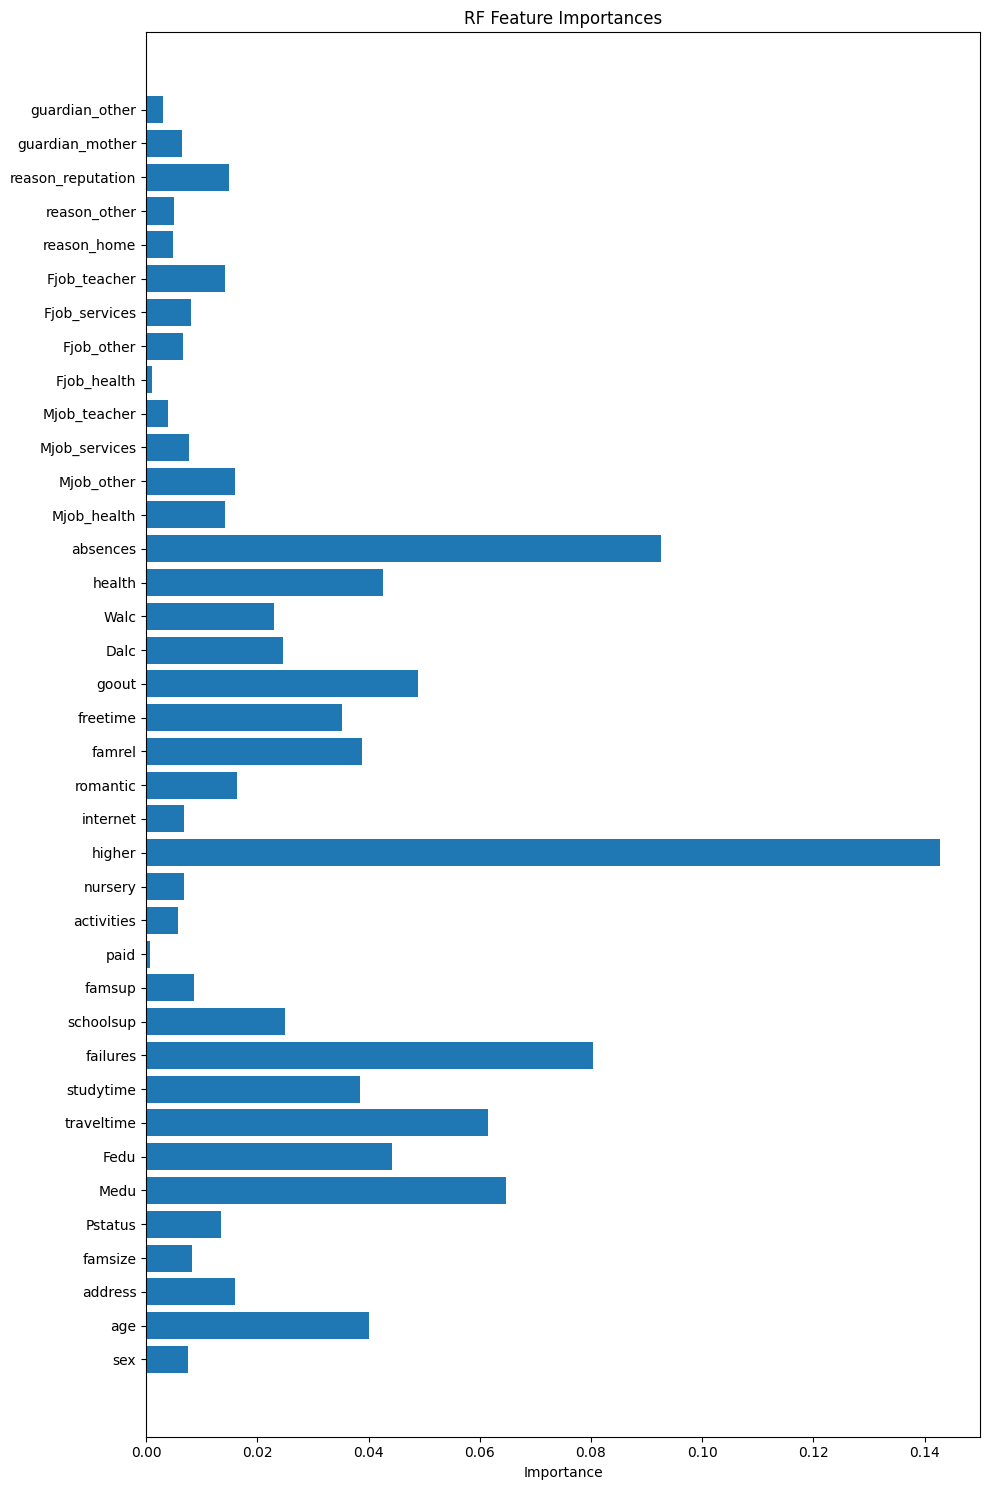
\includegraphics[width=13cm]{init_rf_featimp.png}
\caption{Initial Random Forest Feature Importance when predicting G3}
\label{fig:initrffeatureimportance}
\end{figure}

From the figure, we can see that multiple features like higher, absences, and failures are important when predicting G3, but some features are also not as important. Utilizing this observation, we decided to drop the features were below 0.025 importance, and between -0.1 and 0.1 correlation. All of the features listed below were dropped using the mentioned method:
\begin{itemize}
    \item sex
    \item famsize
    \item Pstatus
    \item famsup
    \item paid
    \item activities
    \item nursery
    \item Mjob\_services
    \item Mjob\_teacher
    \item Fjob\_health
    \item Fjob\_other
    \item Fjob\_services
    \item Fjob\_teacher
    \item reason\_home
    \item reason\_other
    \item guardian\_mother
    \item guardian\_other
\end{itemize}

Building on top of this, we also conducted some feature engineering where we combined Medu and Fedu into one feature: Parental Education where we just got the mean for the two features. Other than that, we also engineered another feature called Total Alcohal Consumption where we combined Dalc and Walc with its respective weights (5/7 and 2/7). After all of this, our list of features can be seen in the table below.

\begin{table}[H]
\centering
\begin{tabular}{|p{4cm}|p{11cm}|}
\hline
Feature & Details \\ \hline
age & student's age (numeric: from 15 to 22)\\ \hline
address & student's home address type (binary: 'U' - urban or 'R' - rural)\\ \hline
parental\_edu & Parents' education (numeric: 0 - none, 1 - primary education (4th grade), 2 - 5th to 9th grade, 3 - secondary education or 4 - higher education)\\ \hline
traveltime & home to school travel time (numeric: 1 - <15 min., 2 - 15 to 30 min., 3 - 30 min. to 1 hour, or 4 - >1 hour) \\ \hline
studytime &  weekly study time (numeric: 1 - <2 hours, 2 - 2 to 5 hours, 3 - 5 to 10 hours, or 4 - >10 hours) \\ \hline
schoolsup & extra educational support (binary: yes or no) \\ \hline
higher & wants to take higher education (binary: yes or no) \\ \hline
internet & Internet access at home (binary: yes or no) \\ \hline
romantic &  with a romantic relationship (binary: yes or no) \\ \hline
famrel & quality of family relationships (numeric: from 1 - very bad to 5 - excellent) \\ \hline
freetime & free time after school (numeric: from 1 - very low to 5 - very high) \\ \hline
goout & going out with friends (numeric: from 1 - very low to 5 - very high) \\ \hline
total\_alcohol & total alcohol consumption (numeric: from 1 - very low to 5 - very high) \\ \hline
health & current health status (numeric: from 1 - very bad to 5 - very good) \\ \hline
absences & number of school absences (numeric: from 0 to 93) \\ \hline
Mjob\_health & Mother's job in healthcare \\ \hline
Mjob\_other & Mother's job in other fields \\ \hline
reason\_reputation & choosing this school due to its reputation \\ \hline
G3 & final grade (numeric: from 0 to 20, output target) \\ \hline
\end{tabular}
\caption{Final Dataset Features and their information after EDA and Feature Engineering}
\label{tab:finalfeatures}
\end{table}


\subsection{Models}
\label{subsec:models}
% Describe each model you implemented in detail
% Explain the architecture, parameters, and hyperparameters
% Justify your model selection
% Include mathematical formulations where appropriate
Our results for the regression models were not great so we'll briefly touch on them in section \ref{subsub:regressionmodels}, and go over each classification model in detail in the following sections.

\subsubsection{Regression Models (1-4)}
\label{subsub:regressionmodels}
We tried the following models with their hyperparameters:
\begin{itemize}
    \item Linear Regression: default hyperparameters
    \item Polynomial Regression: degree=1 (after utilizing cross-validation, results can be seen in figure \ref{fig:polydegreecv})
    \item Decision Tree Classifier: n\_estimators=100, max\_depth=6
    \item LASSO Regression: alphas=np.logspace(-3, 3, 100), cv=5, max\_iter=50000
\end{itemize}

The regression models performed terribly with R² scores of around 0.1-0.15 and RMSE scores of around 3. With average differences of 3 and so little of the variance being able to be captured by the models, we pivoted to using classification models.

\subsubsection{Model 5: Logistic Regression}
Hyperparameters - Default

Since we preprocessed our dataset for classification use by splitting G3 into Pass/Fail buckets, we decided that our first classification model should be Logistic Regression, to set a baseline for all models, providing simple and interpretable results with fast training times.

\subsubsection{Model 6: Decision Tree Classifier}
Hyperparameters - criterion:gini, max\_depth:None, min\_samples\_leaf:1, min\_samples\_split:2

We picked Decision Tree Classifier after Logistic Regression due to its capability to handle non-linearity, as well as providing a fast training time to serve as a second baseline after Logistic Regression.

\subsubsection{Model 7: Random Forest Classifier}
Hyperparameters - max\_depth:None, min\_samples\_leaf:1, min\_samples\_split:2, n\_estimators:300

After deciding to move into more complex models with higher training times, Random Forest was the first that we tried since it can help reduce overfitting and is an improvement from single decision trees. It can also help provide feature importance which is relevant to our research question.

\subsubsection{Model 8: Gradient Boosting Classifier}
Hyperparameters - learning\_rate:0.1, max\_depth:None, min\_samples\_leaf:4, min\_samples\_split:10, n\_estimators:500

We wanted to utilize boosting techniques for better predictions at the cost of training time, so the first boosting method we tried was Gradient Boosting with hopes of a higher accuracy and more details on specific patterns in the trees (even though we ended up not finding any observations on this part).

\subsubsection{Model 9: Extreme Gradient Boosting Classifier}
Hyperparameters - learning\_rate:1, max\_depth:10, n\_estimators:500

As an improvement from Gradient Boosting, we looked into Extreme Gradient Boosting for its faster training time from online sources, and its capability to control overfitting as well.

\subsection{Training and Evaluation Methodology}
% Explain your training process
% Describe cross-validation methods
% List evaluation metrics and justify their selection
% Explain how you compared different models
For all classification models, we preprocessed the dataset to increase model performance and convert it for classification use. First, the G3 target is transformed into knowledge\_gain where a G3 score of 10 or higher is converted to a Pass and anything less is a Fail. Second, 5th and 95th percentile outliers are removed to increase boosting performance. Last, since the Pass class is oversampled from previous iterations of our models, we use RandomOverSampler to oversample Fail in turn to prevent a class imbalance. We also used scikitlearn's GridSearchCV (code snippet can be seen in section \ref{sec:code}) for Decision Tree Classifier, Random Forest Classifier, Gradient Boosting Classifier and Extreme Gradient Boosting Classifier to look for the best hyperparameters. As for evaluation, we utilized the classification report and confusion matrix (listed in section \ref{subsec:modeleval}) to measure the model performance and look for any improvements we can implement.

\section{Results}
\label{sec:results}
% Present your findings clearly with appropriate visualizations
% Analyze the performance of each model
% Compare models using your evaluation metrics
In this section, we'll present each classification model's accuracy, classification reports and confusion matrix, provide some analysis and observations we made, and explain the reason behind picking our final model.

\subsection{Model Evaluation (for Models 5 to 9)}
\label{subsec:modeleval}
Some initial problems we encountered from our previous iterations were misclassification of Fail predictions due to class imbalance. We implemented some fixes but ultimately decided that oversampling Fail was the best approach to address this problem. Below are the Accuracy, Classification Reports and Confusion Matrix for all classification models we utilized, along with some observations we made for each model.

\subsubsection{Model 5: Logistic Regression}
Accuracy: 0.5833
\begin{table}[H]
    \centering
    \begin{tabular}{lcccc}
        \hline
        & \textbf{precision} & \textbf{recall} & \textbf{f1-score} & \textbf{support} \\
        \hline
        0 & 0.57 & 0.69 & 0.62 & 54 \\
        1 & 0.60 & 0.48 & 0.54 & 54 \\
        \hline
        \textbf{accuracy} & & & 0.58 & 108 \\
        \textbf{macro avg} & 0.59 & 0.58 & 0.58 & 108 \\
        \textbf{weighted avg} & 0.59 & 0.58 & 0.58 & 108 \\
        \hline
    \end{tabular}
    \caption{Decision Tree Classification Report}
    \label{tab:lrclassification_report}
\end{table}
\begin{table}[H]
    \centering
    \begin{tabular}{|c|c|c|}
        \hline
        & Predicted Pass & Predicted Fail \\ \hline
        Actual Pass & 37 & 17 \\ \hline
        Actual Fail& 28 & 26 \\ \hline
    \end{tabular}
    \caption{Decision Tree Confusion Matrix}
    \label{tab:lrconfusion_matrix}
\end{table}

We tried out logistic regression to compare with other decision tree and ensemble methods, which we will analyze in the following sections, but this model performed poorly compared to them in every metric with a poor accuracy of 58.33\% and poor predictions as seen from the Classification Report and Confusion Matrix. It serves as a baseline to the later model's performance, and due to this, we decided to not include Logistic Regression when comparing our final models.

% Present detailed results for each model
% Include tables, charts, and graphs to illustrate performance
% Discuss interesting patterns or outliers
\subsubsection{Model 6: Decision Tree Classifier}
Accuracy: 0.8981
\begin{table}[H]
    \centering
    \begin{tabular}{lcccc}
        \hline
        & \textbf{precision} & \textbf{recall} & \textbf{f1-score} & \textbf{support} \\
        \hline
        0 & 0.83 & 1.00 & 0.91 & 54 \\
        1 & 1.00 & 0.80 & 0.89 & 54 \\
        \hline
        \textbf{accuracy} & & & 0.90 & 108 \\
        \textbf{macro avg} & 0.92 & 0.90 & 0.90 & 108 \\
        \textbf{weighted avg} & 0.92 & 0.90 & 0.90 & 108 \\
        \hline
    \end{tabular}
    \caption{Decision Tree Classification Report}
    \label{tab:dtclassification_report}
\end{table}
\begin{table}[H]
    \centering
    \begin{tabular}{|c|c|c|}
        \hline
        & Predicted Pass & Predicted Fail \\ \hline
        Actual Pass & 54 & 0 \\ \hline
        Actual Fail& 11 & 43 \\ \hline
    \end{tabular}
    \caption{Decision Tree Confusion Matrix}
    \label{tab:dtconfusion_matrix}
\end{table}

We can see that due to GridSearchCV, our accuracy is decently high at around 89.81\%. From the confusion matrix, we can also see that our Pass prediction is fully accurate, but the model has some problems predicting Fails correctly even after oversampling it. This is also an improvement from the Logistic Regression model.

\subsubsection{Model 7: Random Forest Classifier}
Accuracy: 0.9444
\begin{table}[H]
    \centering
    \begin{tabular}{lcccc}
        \hline
        & \textbf{precision} & \textbf{recall} & \textbf{f1-score} & \textbf{support} \\
        \hline
        \textbf{0} & 0.90 & 1.00 & 0.95 & 54 \\
        \textbf{1} & 1.00 & 0.89 & 0.94 & 54 \\
        \hline
        \textbf{accuracy} & & & 0.94 & 108 \\
        \textbf{macro avg} & 0.95 & 0.94 & 0.94 & 108 \\
        \textbf{weighted avg} & 0.95 & 0.94 & 0.94 & 108 \\
        \hline
    \end{tabular}
    \caption{Random Forest Classification Report}
    \label{tab:rfclassification_report}
\end{table}
\begin{table}[H]
    \centering
    \begin{tabular}{|c|c|c|}
        \hline
        & Predicted Pass & Predicted Fail \\ \hline
        Actual Pass & 54 & 0 \\ \hline
        Actual Fail & 6 & 48 \\ \hline
    \end{tabular}
    \caption{Random Forest Confusion Matrix}
    \label{tab:rfconfusion_matrix}
\end{table}
Comparing to our Decision Tree Model, our accuracy rose to a very high 94.44\% with great results from our classification report. It also only misclassified six fails as seen from the Confusion Matrix.

\subsubsection{Model 8: Gradient Boosting Classifier}
Accuracy: 0.9074
\begin{table}[H]
    \centering
    \begin{tabular}{lcccc}
        \hline
        & \textbf{precision} & \textbf{recall} & \textbf{f1-score} & \textbf{support} \\
        \hline
        \textbf{0} & 0.84 & 1.00 & 0.92 & 54 \\
        \textbf{1} & 1.00 & 0.81 & 0.90 & 54 \\
        \hline
        \textbf{accuracy} & & & 0.91 & 108 \\
        \textbf{macro avg} & 0.92 & 0.91 & 0.91 & 108 \\
        \textbf{weighted avg} & 0.92 & 0.91 & 0.91 & 108 \\
        \hline
    \end{tabular}
    \caption{Gradient Boosting Classification Report}
    \label{tab:gbclassification_report}
\end{table}
\begin{table}[H]
    \centering
    \begin{tabular}{|c|c|c|}
        \hline
        & Predicted Pass & Predicted Fail \\ \hline
        Actual Pass & 54 & 0 \\ \hline
        Actual Fail& 10 & 44 \\ \hline
    \end{tabular}
    \caption{Gradient Boosting Confusion Matrix}
    \label{tab:gbconfusion_matrix}
\end{table}
Grading Boosting proved to be more effective than Decision Tree Classifier, but still performed worse than RandomForest, with a lower accuracy of 90.74\% and misclassifying 10 fails as seen from the Confusion Matrix.

\subsubsection{Model 9: Extreme Gradient Boosting Classifier}
Accuracy: 0.9352
\begin{table}[H]
    \centering
    \begin{tabular}{lcccc}
        \hline
        & \textbf{precision} & \textbf{recall} & \textbf{f1-score} & \textbf{support} \\
        \hline
        \textbf{0} & 0.89 & 1.00 & 0.94 & 54 \\
        \textbf{1} & 1.00 & 0.87 & 0.93 & 54 \\
        \hline
        \textbf{accuracy} & & & 0.94 & 108 \\
        \textbf{macro avg} & 0.94 & 0.94 & 0.93 & 108 \\
        \textbf{weighted avg} & 0.94 & 0.94 & 0.93 & 108 \\
        \hline
    \end{tabular}
    \caption{Extreme Gradient Boosting Classification Report}
    \label{tab:xgbclassification_report}
\end{table}
\begin{table}[H]
    \centering
    \begin{tabular}{|c|c|c|}
        \hline
        & Predicted Pass & Predicted Fail \\ \hline
        Actual Pass & 54 & 0 \\ \hline
        Actual Fail& 7 & 47 \\ \hline
    \end{tabular}
    \caption{Extreme Gradient Boosting Confusion Matrix}
    \label{tab:xgbconfusion_matrix}
\end{table}
Extreme Gradient Boosting provided similar results as our RandomForest model, with an accuracy of 93.52\% and misclassifying seven fails compared to the six of RandomForest. This is very comparable to the RandomForest model in terms of performance and accuracy when it comes to predictions.

\subsection{Comparative Analysis}
% Compare all models side by side
% Analyze strengths and weaknesses of each approach
% Identify the best-performing model and explain why it performed well
\begin{figure} [H]
\centering % Centers the figure in the middle of the page
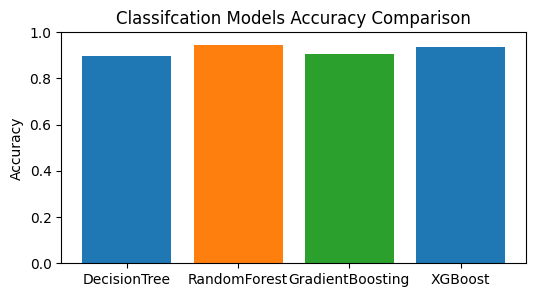
\includegraphics[width=9cm]{classification_model_comparison.png}
\caption{Accuracy Comparison of our four models after dropping Logistic Regression}
\label{fig:modelacccomparison}
\end{figure}

From the figure above, we can see that RandomForest and XGBoost come out on top as the two highest accuracy, and from our model evaluation in section \ref{subsec:modeleval}, we also observed that RandomForest and XGBoost predicts Fail better than the other two. We'll pick those two and compare the feature importance from both models in the figure below.

\begin{figure}[H]
  \centering
  \begin{minipage}[b]{0.45\textwidth}
    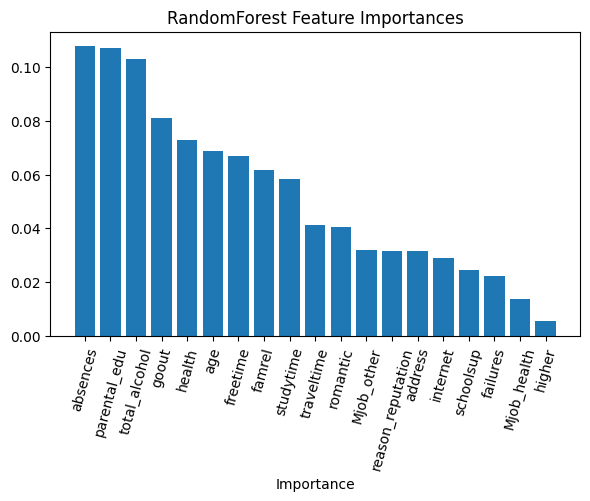
\includegraphics[width=\textwidth]{rf_fimp.png}
  \end{minipage}
  \hfill
  \begin{minipage}[b]{0.45\textwidth}
    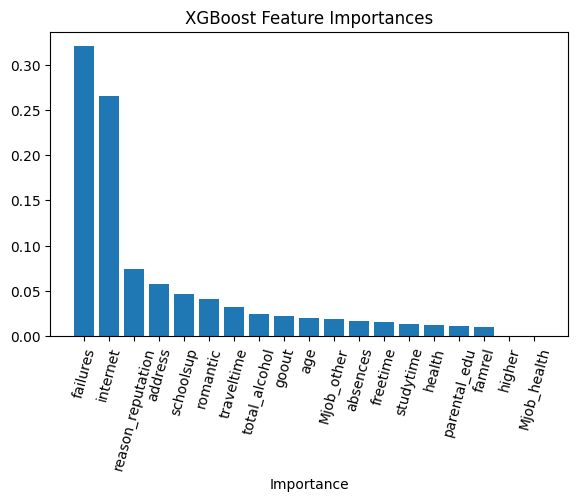
\includegraphics[width=\textwidth]{xgboost_fimp.png}
  \end{minipage}
  \caption{RandomForest and XGBoost Feature Importance Comparison}
\end{figure}

From the comparison, we can see that RandomForest highlights absences, parental\_edu, and total\_alcohol as the top three features that stand above the rest, and XGBoost highlights failures and internet as the top two features. With these two observations, we can conclude that both RandomForest and XGBoost give valuable insight into the most important features and the five most important features that has an impact on students' academic performance are the number of failures the student has in the past, internet access, absences, education level of parents, and total alcohol consumption.

\section{Discussion}
% Interpret your results in the context of your research question(s)
% Explain what your findings mean for the problem domain
From section \ref{sec:results}, we found that the two best performing models are RandomForest and XGBoost, with both providing insightful observations to our research question, what best predicts a student's academic performance. The final five features we decided on are the number of failures the student has in the past, internet access, absences, education level of parents, and total alcohol consumption.

The number of failures the student has in the past makes a lot of sense in this context since that shows the student's performance in the past, but this doesn't really provide much information on what should be improved from a student's perspective, but it does confirm that a student with a poor track record must put in the work to improve. Internet access and education level of parents is a bit more helpful, in the context of how the student learns. Since our dataset relies on secondary school students (where parents tend to tutor their students), it may show that having parents that are more educated can lead to more effective teaching methods that are easier for students to understand. On top of this, having internet access can help a student whether they are self-studying, or when they need information on anything. This might have some downsides especially since the internet can have many distractions and when internet usage is not supervised, using it for learning can become ineffective.

Features like absences and alcohol consumption also makes sense since classes are the primary way for a student to learn course material so missing classes can lead to gaps in knowledge, resulting in lower grades. Alcohol consumption is also a topic discussed widely, especially for college students, where alcohol abuse interferes with a student's sleep, study pattern and can cause addiction. These two negative features can be used to incentivize students to not miss class and not abuse addictive substances.

\subsection{Connections to Prior Work}
% Compare your results with existing literature
From Cortez et al.'s paper, they found that number of absences, parent’s jobs and education, and alcohol consumption levels are important \cite{cortez2008using}. This matches with up our findings as well, even though we took a different machine learning approach, and shows the importance of attending classes, not consuming alcohol, having access to the internet, and the level of education of parents when it comes to a student's academic performance. Of course, we understand that a student cannot do anything about their parents' education, but with dedication to learning (through classes or online/self-studying) and the willingness to stay away from addictive substances, it can help greatly with their academic performance. 

\subsection{Limitations}
% Discuss limitations of your approach
We are aware that this is just using one dataset, with a somewhat small sample size of 382. This may not represent accurate results when utilizing a dataset with different features, but the observations we made can still prove to be useful.

\section{Conclusion \& Future Work (0.5 page)}
% Summarize your key findings and contributions
% Relate back to your research question(s)
% Suggest directions for future research
% Discuss potential improvements or extensions to your work
In this paper, we answered our research question, ``What best predicts a student's academic performance", using different machine learning techniques like regression and classification models. After testing around with many models and techniques(like Cross-Validation, GridSearchCV, Boosting, and Oversampling), we concluded that our RandomForest and Extreme Gradient Boosting models were the best in terms of prediction accuracy and performance. Using the two models, we drew the conclusion(from feature importance in the predictions) that number of failures the student has in the past, internet access, absences, education level of parents, and total alcohol consumption are the most important when it comes to predicting a student's grade. The four features (apart from education level of parents) are what students should be focusing on when aiming to achieving higher grades.

For future work, we recommend taking a similar approach with multiple dataset that includes different features, and perform a comparison of observations made at the end. Comparing the most impactful features and seeing if some of them overlap can help narrow down which ones to focus on from a student's perspective, as well as provide insightful information for academic institutions to help better assist students.

\section*{Acknowledgments}
% (Optional) Acknowledge any assistance or resources that supported your project
We are deeply grateful to our Professor Kelsey Urgo, for all of the assistance in the project as well as Professor Alark Joshi for introducing us to Overleaf so that our report looks as good as it does. We also would like to thank Cortez et al., and Aman Chauhan for providing former research on the field and the dataset that we used for our research.

\bibliographystyle{plainnat}
\bibliography{references}
% Create a references.bib file with your citations

\appendix
\section{Appendix: Additional Visualizations}
\label{sec:addvis}
% Include additional figures, tables, or analyses that support but are not essential to the main text
\begin{figure} [H]
\centering % Centers the figure in the middle of the page
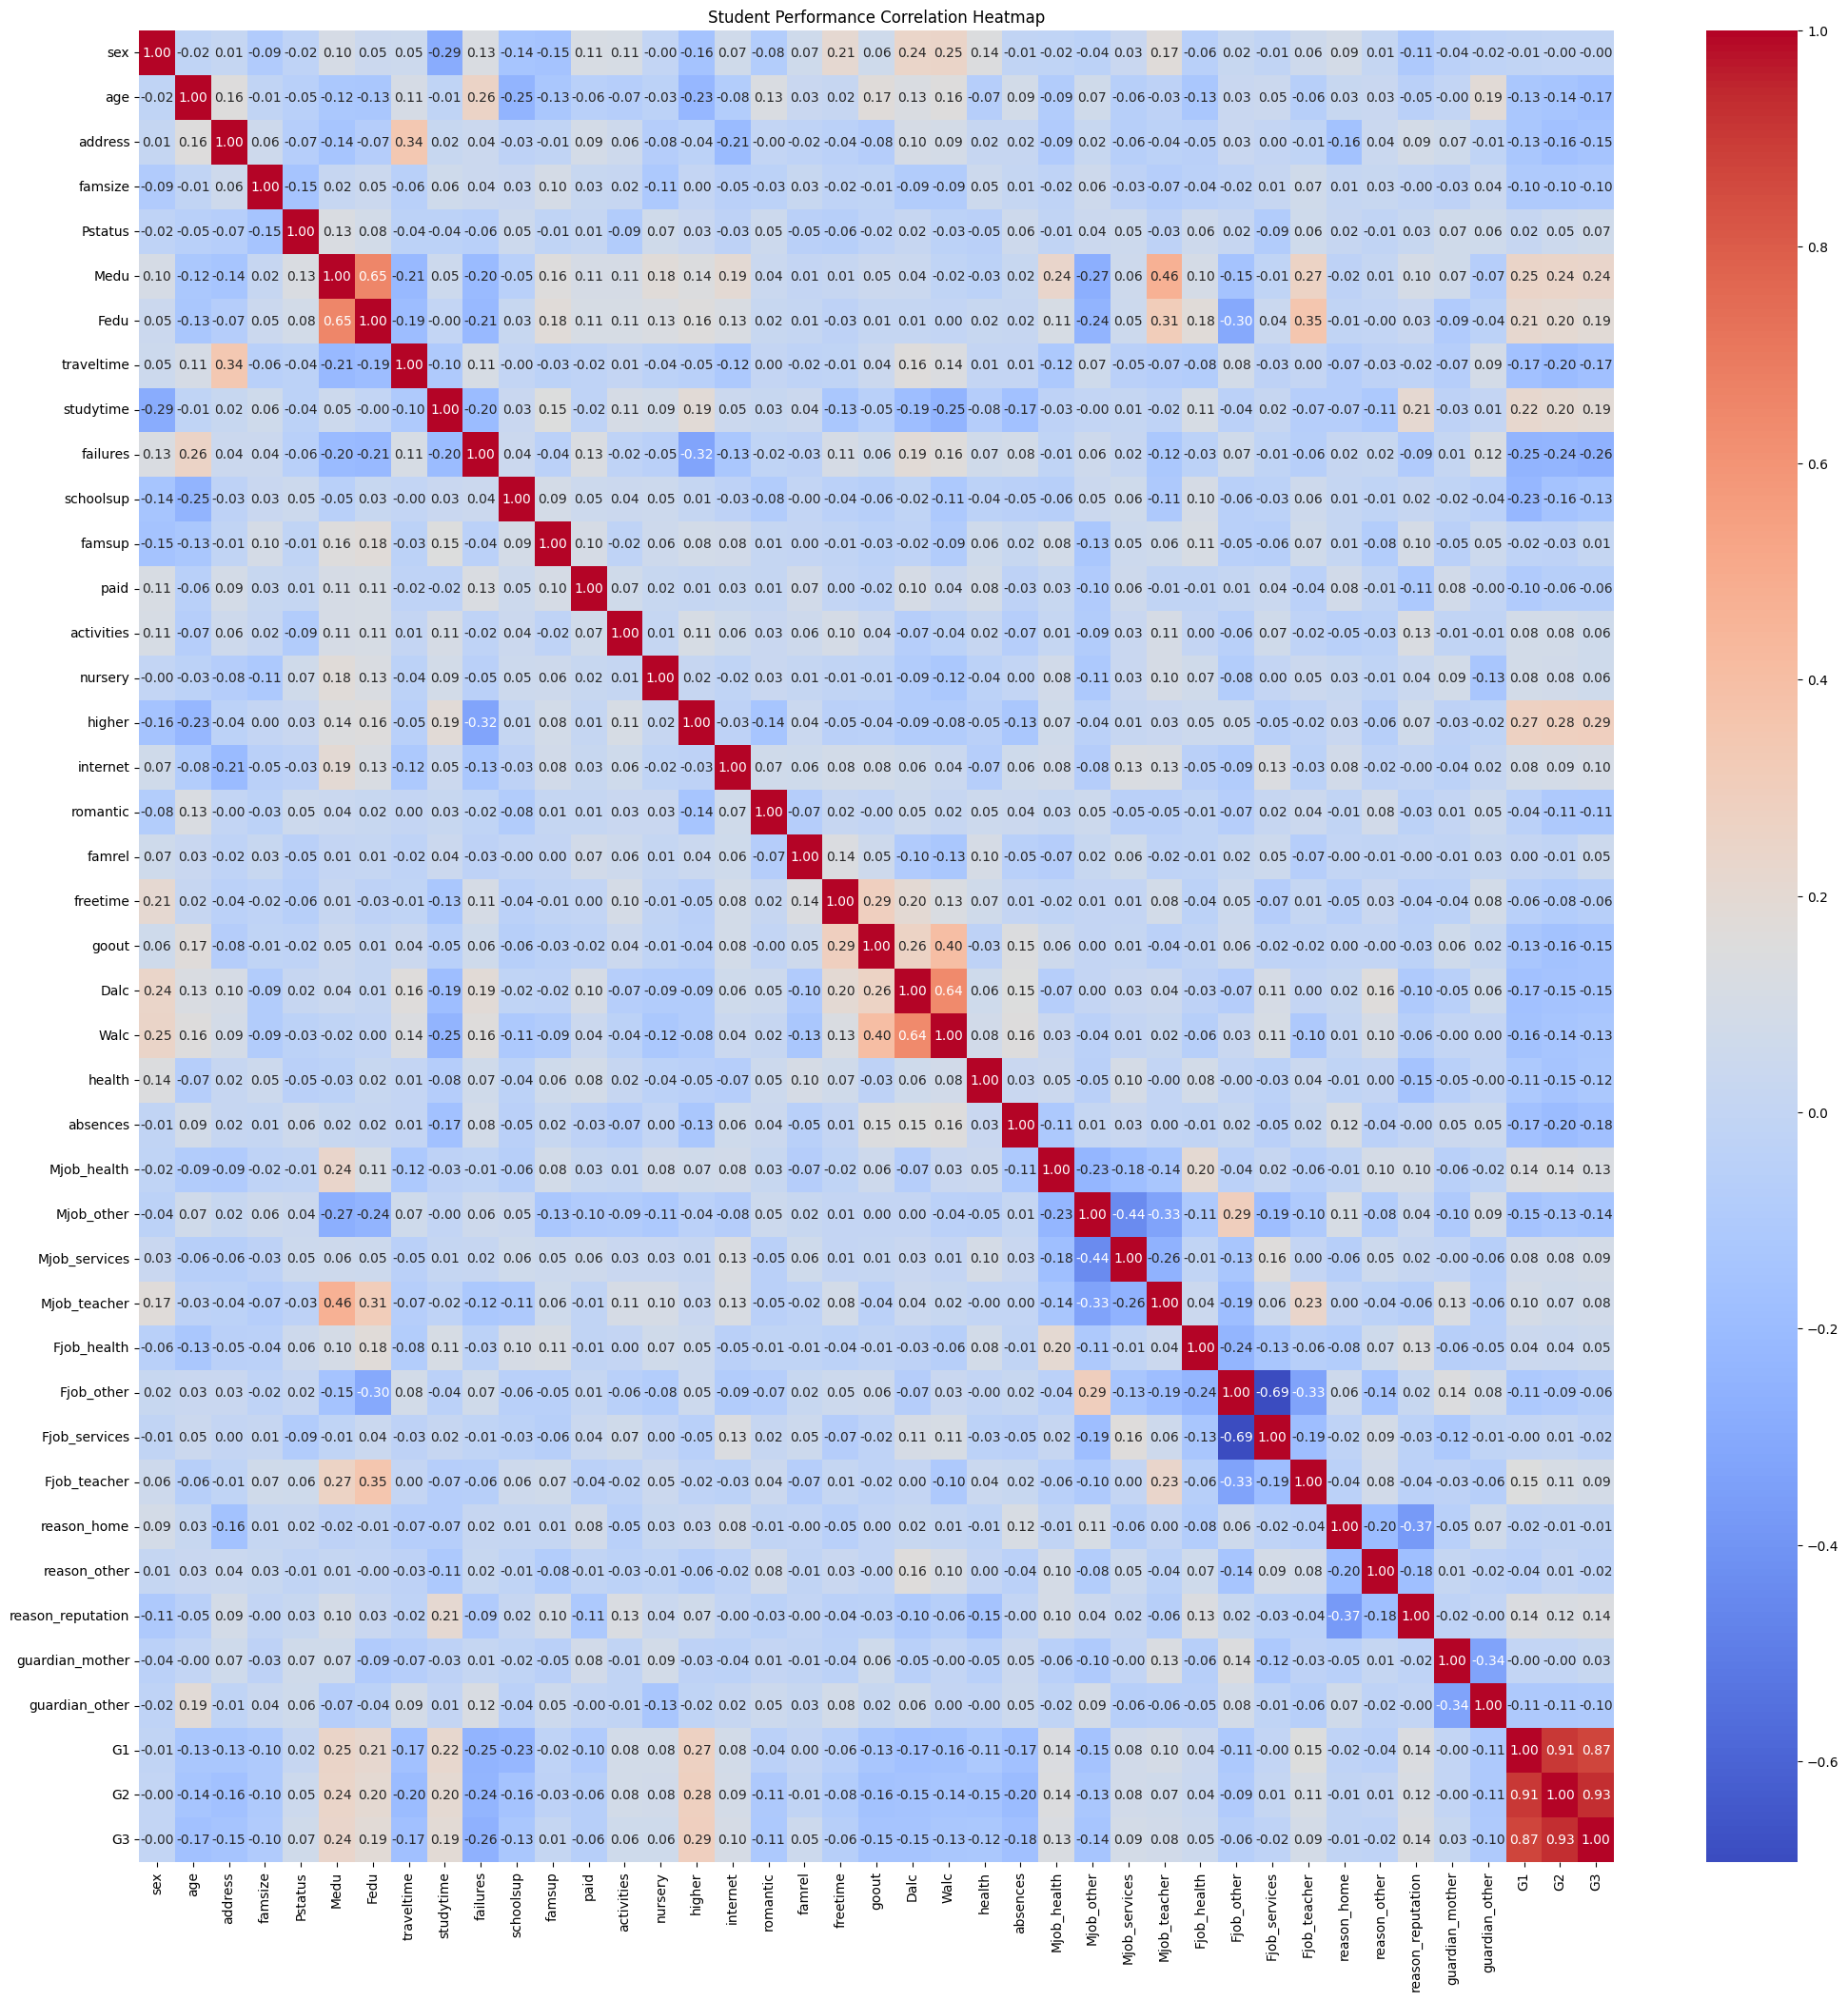
\includegraphics[width=15cm]{init_heatmap.png}
\caption{Initial Feature Correlation Heatmap of the dataset}
\label{fig:initheatmap}
\end{figure}

\begin{figure} [H]
\centering % Centers the figure in the middle of the page
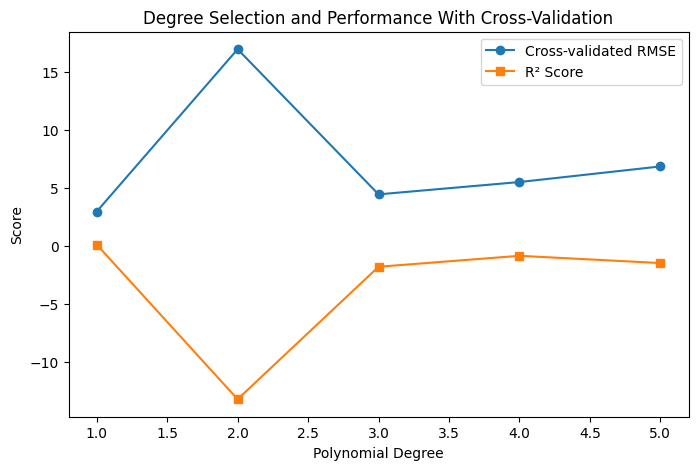
\includegraphics[width=15cm]{poly_degree_cv.png}
\caption{Using Cross-Validation to find best Polynomial degree}
\label{fig:polydegreecv}
\end{figure}

\section{Appendix: Code Implementation Details}
\label{sec:code}
% Include snippets of especially important code
% Explain any complex algorithms or implementation details
% Provide information on how to access the full code repository
\begin{lstlisting}[language=Python, caption=Encoding Code Snippet]
# One hot encoding
df = pd.get_dummies(df, columns=['Mjob', 'Fjob', 'reason', 'guardian'], drop_first=True)
# Converting categorical variables into numericals + dropping unnecessary columns
df = df.drop(columns=['school']) # Dropping school since school location should not affect much in our scope
df['sex'] = df['sex'].map({'F': 0, 'M': 1}) # Female: 0, Male: 1
df['address'] = df['address'].map({'U': 0, 'R': 1}) # Urban: 0, Rural: 1
df['famsize'] = df['famsize'].map({'LE3': 0, 'GT3': 1}) # Less than or equal to 3: 0, Greater than 3: 1
df['Pstatus'] = df['Pstatus'].map({'T': 0, 'A': 1}) # Together: 0, Apart: 1
df['schoolsup'] = df['schoolsup'].map({'no': 0, 'yes': 1}) # Extra educational support: 0 if no, 1 if yes
df['famsup'] = df['famsup'].map({'no': 0, 'yes': 1}) # Family educational support: 0 if no, 1 if yes
df['paid'] = df['paid'].map({'no': 0, 'yes': 1}) # Extra paid classes: 0 if no, 1 if yes
df['activities'] = df['activities'].map({'no': 0, 'yes': 1}) # Extracurricular activities: 0 if no, 1 if yes
df['nursery'] = df['nursery'].map({'no': 0, 'yes': 1}) # Attended nursery school: 0 if no, 1 if yes
df['higher'] = df['higher'].map({'no': 0, 'yes': 1}) # Wants to take higher education: 0 if no, 1 if yes
df['internet'] = df['internet'].map({'no': 0, 'yes': 1}) # Internet access at home: 0 if no, 1 if yes
df['romantic'] = df['romantic'].map({'no': 0, 'yes': 1}) # With a romantic relationship: 0 if no, 1 if yes
\end{lstlisting}


\begin{lstlisting}[language=Python, caption=Using GridSearchCV for best hyperparameters for Classification models]
param_grid_dtc = {
    'criterion': ['gini', 'entropy'],
    'max_depth': [None, 2, 5, 10],
    'min_samples_split': [2, 5, 10],
    'min_samples_leaf': [1, 2, 4],
}
param_grid_rfc = {
    'n_estimators': [50, 100, 300, 500],
    'max_depth': [None, 2, 5, 10],
    'min_samples_split': [2, 5, 10],
    'min_samples_leaf': [1, 2, 4],
}
param_grid_gb = {
    'n_estimators': [50, 100, 300, 500],
    'max_depth': [None, 2, 5, 10],
    'min_samples_split': [2, 5, 10],
    'min_samples_leaf': [1, 2, 4],
    'learning_rate': [1, 0.1, 0.01, 0.001],
}
param_grid_xgb = {
    'n_estimators': [50, 100, 300, 500],
    'max_depth': [None, 2, 5, 10],
    'learning_rate': [1, 0.1, 0.01, 0.001],
}
# Find the best hyperparameters for every model
gs_dtc = GridSearchCV(DecisionTreeClassifier(random_state=42), param_grid_dtc, cv=5, n_jobs=-1, scoring='f1')
gs_rfc = GridSearchCV(RandomForestClassifier(random_state=42), param_grid_rfc, cv=5, n_jobs=-1, scoring='f1')
gs_gb = GridSearchCV(GradientBoostingClassifier(random_state=42), param_grid_gb, cv=5, n_jobs=-1, scoring='f1')
gs_xgb = GridSearchCV(xgb.XGBClassifier(random_state=42), param_grid_xgb, cv=5, n_jobs=-1, scoring='f1')
\end{lstlisting}

\end{document}